% !TeX root = e4_tp1_ej2
\documentclass[e4_tp1_main.tex]{subfiles}

\begin{document}

\section{Ejercicio 2}

\begin{wrapfigure}[10]{R}{0.4\textwidth}
	\centering
	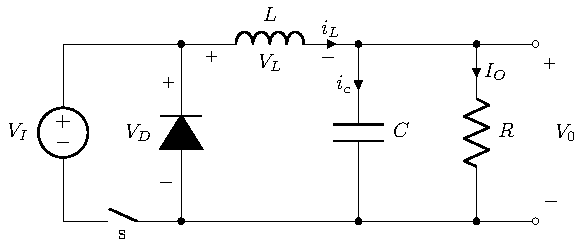
\includegraphics[width=0.4\textwidth]{images/ej2/buck_ideal.pdf}
	\caption{Fuente buck con llave ideal}
	\label{fig:buck-ideal}
\end{wrapfigure}

El circuito que analizaremos ahora es una fuente buck, es decir, un convertidor DC/DC donde la tensi\'on de salida es menor que la de entrada. El mismo puede observarse en la figura \ref{fig:buck-ideal}. En esta secci\'on, consideraremos ideal a la llave con la que se hace el switching.
Los requeriminetos que debe cumplir esta fuente son: $V_I$ = 9.0V, $V_O$ = 3.7V, $\nicefrac{\Delta V_O}{V_O}_{max}$ = 5\%.


Esto se debe lograr a una frecuencia de switching de $f_s = 50$kHz. En cuanto a los componentes pasivos, los reactivos son sugeridos por la c\'atedra: $L=220\upmu$H y $C=10\upmu$F. La resistencia de carga  debe ser elegida de manera tal que, en primera instancia, la fuente funcione en modo continuo.



\subsection{An\'alisis te\'orico}

\subsubsection{Con componentes ideales}

Para obtener la salida indicada, debemos seleccionar el duty adecuado. Esto se puede obtener planteando que en r\'egimen permanente, $\langle V_L \rangle = 0$, y por lo tanto, $\langle V_O \rangle = \langle V_D \rangle$. Considerando al diodo como ideal, su tensi\'on es 0 cuando la llave est\'a abierta, y $V_I$ cuando est\'a cerrada. Por lo tanto, despejado para $D$ obtenemos que:
\begin{equation}
	D = \nicefrac{V_O}{V_I} \simeq 0.41
\end{equation}  

Con este valor, podemos ahora obtener la corriente de boundary. Sabiendo que cuando la llave est\'a abierta, $V_L = L \frac{di_L}{dt} = -V_0$, y que esta condici\'on se mantiene por un tiempo $T_s \cdot (1-D)$, se obtiene:
\begin{equation}
	\Delta I_L = \left(\nicefrac{V_O}{L}\right) \cdot (1-D) \cdot T_s \simeq 0.20\text{A}
	\Rightarrow
	I_{B} = \Delta I_L/2 \simeq 0.10\text{A}
\end{equation} 

Para que $I_O > I_B$, elegimos pues $R = 10\Omega$, lo cual resulta en una corriente de salida de 0.37A.

El ripple de tensi\'on, por otro lado, es entonces de:
\begin{equation}
	\nicefrac{\Delta V_O}{V_O} 
	= \left(\nicefrac{1}{V_O}\right) \cdot \left(\nicefrac{\Delta Q}{C}\right) 
	= \left(\nicefrac{1}{V_O}\right) 
	\cdot \left(\nicefrac{1}{C}\right) \cdot \left(\nicefrac{1}{2}\right) \cdot \left(\nicefrac{\Delta I_L}{2}\right) \left(\nicefrac{T_s}{2}\right)
	\simeq 1.23 \%	
	\label{eq:ripple1}
\end{equation}

Este valor se encuentra por debajo del m\'aximo aceptable de 5\%.


\subsubsection{Considerando la tensi\'on forward del diodo}

El an\'alisis anterior sirve como primera aproximaci\'on del comportamiento del circuito. Sin embargo, a la hora de simular, resulta evidente que no es suficiente: la tensi\'on obtenida a la salida es considerablemente menor a la que se requiere, de alrededor de 3.2V.

En primer lugar, podemos observar que si bien es cierto que $V_O = \langle V_D \rangle$, en la secci\'on anterior consideramos que cuando la llave est\'a cerrada, la tensi\'on en el diodo es nula. Sin embargo, sabemos que esto no es cierto: el diodo estar\'a forward-biased, con lo cual su tensi\'on no ser\'a otra que la de forward. De la datasheet del 
MUR460\footnote{
	\url{https://www.onsemi.com/pub/Collateral/MUR420-D.PDF}
}, consultando las figuras 6 (tensi\'on forward en funci\'on de corriente forward y temperatura), 9 (potencia disipada en funci\'on de corriente forward y forma de onda), se llega a la conclusi\'on de que la tensi\'on forward del diodo rondar\'a los $V_{FD}= 0.8$V.

Una vez que contamos con este valor, podemos calcular el nuevo valor de la tensi\'on de salida: 
\begin{equation}
	V_O = \langle V_D \rangle = D \cdot V_I - (1-D) \cdot V_{DF}   
\end{equation}

Despejando para $D$, obtenemos:
\begin{equation}
	D = (V_O + V_{DF})/(V_I + V_{DF}) 
	= (3.7V + 0.8V)(9V + 0.8V)
	\simeq 0.46 
\end{equation}

Esto a su vez cambiar\'a el valor de los ripples de tensi\'on y corriente, puesto que no s\'olo a la tensi\'on de la bobina durante $T_{off}$ se le suma la tensi\'on forward del diodo, sino que adem\'as al aumentar $D$, disminuye $T_{off}$. Resulta entonces: 
\begin{equation}
	\Delta I_L = (V_O + V_{DF}) \cdot (1-D) \cdot T_s / L
	\simeq 0.21\text{A}
\end{equation} 

Con este valor, la corriente de boundary sube a 0.11A, con lo cual a\'un seguimos operando en modo continuo con 10$\Omega$ de carga. En cuanto al ripple de tensi\'on, utilizando la ecuaci\'on \ref{eq:ripple1} con el nuevo valor de $\Delta I_L$, es 1.53\%.


\subsubsection{Considerando las ESR de la bobina y el capacitor}

Si tenemos en cuenta las ESR, el circuito queda con la configuraci\'on que se observa en la figura \ref{fig:buck-esrs}.

\begin{wrapfigure}[13]{R}{0.5\textwidth}
	\centering
	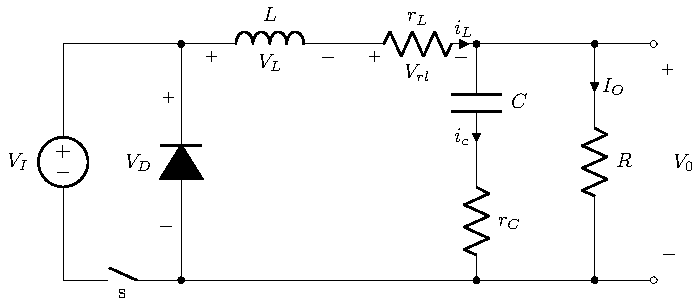
\includegraphics[width=0.5\textwidth]{images/ej2/buck_esrs.pdf}
	\caption{Fuente buck, considerando las ESR de la bobina y del capacitor}
	\label{fig:buck-esrs}
\end{wrapfigure}


Para seguir cumpliendo con $\langle V_L \rangle = 0$, debe cumplirse ahora que $\langle V_D \rangle = \langle V_O \rangle + \langle V_{rL} \rangle$. Como la corriente media de la bobina es la de salida, la tensi\'on media de su ESR no ser\'a otra cosa que $\frac{r_L}{R} \cdot V_O$. 

La datasheet de la bobina sugerida por la 
c\'atedra\footnote{
	\url{https://abracon.com/Magnetics/radial/AIUR-03.pdf}
} lista a esta ESR con el valor de 0.65$\Omega$.
Despejando para $D$, obtenemos pues:
\begin{equation}
	D = \left(V_O \cdot \left( 1+ \frac{r_L}{R}\right)+ V_{DF}\right)/(V_I + V_{DF}) 
\simeq 0.48 
\end{equation}


El ripple de corriente, despreciando nuevamente $i_C$ y sus cambios frente a $I_O$, ahora es:
\begin{equation}
	\Delta I_L = (V_{DF} + V_O) \cdot (1+\nicefrac{r_L}{R} \cdot (1-D) \cdot T_s / L\simeq 0.22\text{A} 
\end{equation}

En cuanto al ripple de tensi\'on, el mismo se ve afectado por la ESR del capacitor, ya que ahora $V_O = V_C + V_{rC}$, con lo cual los efectos de ambos componentes deben tenerse en cuenta. El \textit{application report} ``Output Ripple Voltage for Buck Switching Regulator'' de Texas Instruments\footnote{ 
	\url{http://www.ti.com/lit/an/slva630a/slva630a.pdf}
} realiza el an\'alisis correspondiente, que si bien no es de gran complejidad, s\'i implica un desarrollo demasiado extenso para incluir en este informe paso por paso. El mismo consiste en obtener la $v_o(t) = v_c(t) + v_{rC}(t)$, para los tramos $t<T_{on}$ y el $t>T_{on}$, derivar para buscar el m\'aximo y el m\'inimo de esa funci\'on por tramos, evaluar en esos puntos y obtener la diferencia. Para nuestro caso, dado que la ESR del capacitor es de 32$\Omega$\footnote{ 
\url{https://ar.mouser.com/datasheet/2/129/rtk_e-6792.pdf}
} como $\uptau = r_c \cdot C > T_{off}/2$ y $\uptau > T_{on}/2$, el resultado al que se llega es: 

\begin{equation}
	\Delta V_O =	\Delta I_L \cdot r_C \simeq 7.04\text{V}
	\label{eq:ripple-real}
\end{equation}

Es claro que esto no es aceptable, y es necesario cambiar el capacitor por uno con menor ESR.

Se propone utilizar un capacitor de la serie ESL de KEMET Electronic Components\footnote{
	\url{https://content.kemet.com/datasheets/KEM_A4074_ESL.pdf}
}, en particular el de 39$\upmu$F, 50V, que tiene 0.23$\Omega$ de ESR. Se obtiene entonces $\uptau = 8.97 \upmu$s, con lo cual se est\'a en el \'ultimo caso de la ecuaci\'on \ref{eq:ripple-real}, y entonces:

\begin{equation}
	\nicefrac{\Delta V_O}{V_O} = \Delta I_L \cdot r_C/V_O = 1.36 \%
	\label{eq:result-ripple-esr}
\end{equation}

Llama la atenci\'on que este resultado es menor al obtenido antes de introducir la ESR. Sin embargo, si se corrigiese por el hecho de que ahora el capacitor es casi cuatro veces m\'as grande, s\'i se estar\'ia obteniendo un resultado menos favorable (aunque m\'as preciso) con esta f\'ormula.


\subsubsection{Considerando la corriente de recovery del diodo}

Un comportamiento no ideal del diodo que no se mencion\'o hasta ahora es su corriente de recovery, a la cual se hizo referencia ya en el ejercicio anterior. Lo que sucede es que como la misma depende de la derivada de la corriente en el diodo cuando se lo apaga, y como la fuente y el switch son ideales, esta derivada es infinita. Esto resulta en que los picos de corriente inversa sean, idealmente, infinitos.

Desde luego, esto no es razonable: sabemos que ninguna fuente ni ninguna llave (y para el caso, ning\'un diodo) tiene la capacidad de entregar corriente infinita. Por lo tanto, para plasmar este fen\'omeno  en nuestro an\'alisis de alguna manera, recurriremos nuevamente a la hoja de datos. Encontramos que cuando $\frac{di_R}{dt} = 50\nicefrac{\text{A}}{\upmu \text{s}}$, con una corriente de forward de 1A (que no es nuestro caso, pero nuevamente, esto es a modo ilustrativo), el tiempo de recovery es como m\'aximo $t_{rr}=75$ns, y la corriente $I_{rr} = 1.7$A. Utilizaremos pues estos datos para construir el pico de corriente inversa que se observar\'ia en la realidad.

La forma que toma la curva de $i_D(t)$ en recovery supera el alcance de este trabajo, y aqu\'i simplemente la graficaremos como si fuese triangular. 



\subsection{Simulaci\'on}

\begin{wrapfigure}[13]{R}{0.4\textwidth}
	\centering
	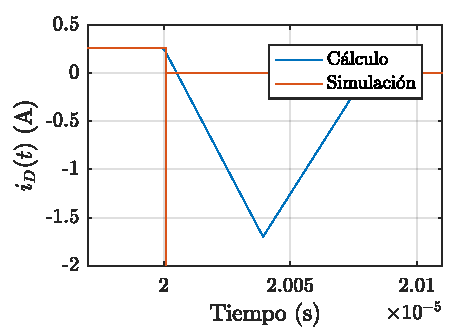
\includegraphics[width=0.35\textwidth]{images/ej2/id-recovery.pdf}
	\caption{Corriente de recovery del diodo}
	\label{fig:id-recovery}
\end{wrapfigure}

Se realizaron las simulaciones correspondientes a este circuito en LTSpice, utilizando el modelo ``real'' del diodo, y con las ESR obtenidas de las datasheets de los componentes correspondientes. Los resultados obtenidos, as\'i como las curvas te\'oricas realizadas a partir del desarrollo de la secci\'on anterior, se encuentran en la figura \ref{fig:buck-curvas}.

En los gr\'afico de $v_L(t)$ e $i_L(t)$ no se observan diferencias significativas entre ambas curvas. Una fuente de error en estas curvas es que Spice utiliza $V_{DF} \simeq 0.77V$, es decir, una tensi\'on un 4\% menor a la que tomamos en el an\'alisis te\'orico. Esto afecta a la tensi\'on de salida, que en la simulaci\'on es de 3.67V. Ambos valores influyen en la cuenta de $v_L$ y, por lo tanto, de $i_L$.



En cuanto a la corriente del diodo, las curvas coinciden la mayor parte del tiempo, lo cual es razonable: en s=0, son iguales a $i_L$, y en $T_{off}$  circula s\'olo la corriente inversa del diodo, que es en el peor caso de 200$\upmu$A y tan peque\~na como 10$\upmu$A (seg\'un la datasheet), y por lo tanto completamente despreciable los \'ordenes de magnitud que estamos trabajando.


Aparece, sin embargo, una gran diferencia en el tiempo de recovery, que se puede apreciar en detalle en la figura \ref{fig:id-recovery}. Esto era lo que esper\'abamos, dado que el switching es ideal, y por lo tanto la derivada de corriente ser\'a tan grande como peque\~no sea el timestep utilizado en la simulaci\'on. El pico obtenido en la simulaci\'on superaba los 200A, pero desde luego este valor no es representativo. 


\begin{figure}[ht]
	\centering
	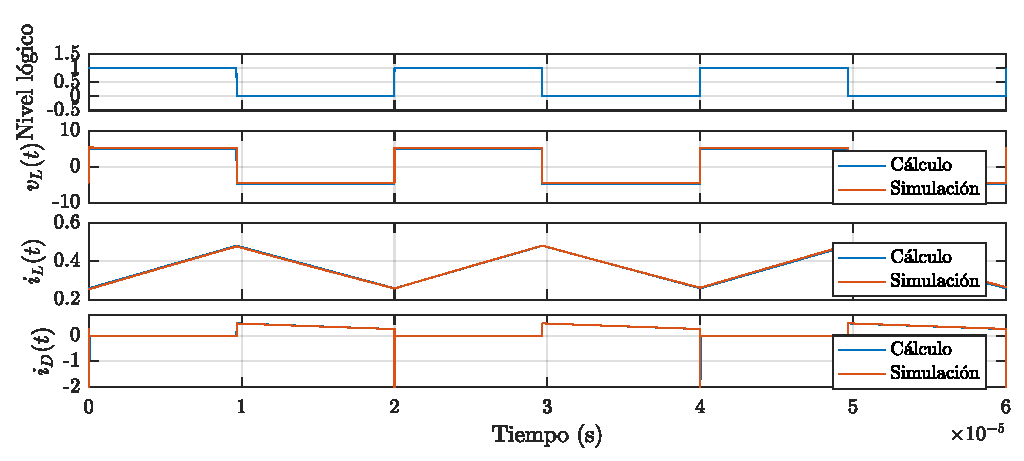
\includegraphics[width=0.75\textwidth]{images/ej2/curvas.pdf}
	\caption{Curvas te\'oricas y simuladas de la fuente buck}
	\label{fig:buck-curvas}
\end{figure}






\end{document}

